\documentclass[11pt,a4paper]{article}
\usepackage[T1]{fontenc}
\usepackage[margin=2.3cm]{geometry}
\usepackage{amsmath,amssymb}
\usepackage{graphicx}
\usepackage[dvipsnames]{xcolor}
\usepackage{enumitem}
\usepackage[colorlinks=true,linkcolor=blue,urlcolor=blue]{hyperref}
\setlength{\parskip}{0.6em}
\setlength{\parindent}{0pt}
\begin{document}

\begin{center}{\LARGE\bfseries openparametric}\\[0.4em]{\large Learn how rules and equations turn requirements into engineered parts, in three sessions.}\\[0.2em]\small PAN IIT OSS explainer \textbullet{} diploma/undergrad to advanced undergrad (levels 2-4)\end{center}

\section*{Why this exists}
Every engineered product is a family of parts that must change when a customer changes the load, the material or the size. This explainer shows how the rules behind such a family are written, ordered, checked and run, which you can build yourself.

\section*{The end goal}
The end goal is to generate engineered parts from rules and equations like computational engineering tools. The same ideas carry over to configurators, to design automation inside CAD programs and to the rule sets of design standards, which have many more rules, units and conditions.

\section*{How the three sessions build up}
\begin{enumerate}[nosep]
\item \textbf{Session 1: From a requirement to a size: a rule and a standard size} (Level 2: mathematical engineering model, 60 min).
\item \textbf{Session 2: When two rules disagree the stricter one wins: strength, stiffness and material} (Level 3: simulation and validation, 75 min).
\item \textbf{Session 3: Rules as data: ordering them, catching loops and drawing the part} (Level 3: simulation and validation, 90 min).
\end{enumerate}

\section{Session 1: From a requirement to a size: a rule and a standard size}

\subsection*{A. Real-world problem}
A motor must turn a machine with a torque of 200 N m. What diameter should the steel shaft have? A designer does not guess: there is a rule that links the torque, the strength of the steel and a safety margin to the smallest safe diameter, and a second rule that rounds it up to a size that can be bought. If the requirement changes, the rules give a new shaft at once. How do such rules work, and how do we know the shaft is safe?

\subsection*{B. Concept and theory}
When a solid round shaft of diameter d carries a torque T, the largest shear stress is at its surface: tau = 16 T / (pi d\textasciicircum{}3), with T in N mm and d in mm giving tau in MPa (N/mm\textasciicircum{}2). The steel may only be loaded to an allowable stress: its shear yield strength, about 0.577 times the tensile yield strength sigma\_y, divided by a safety factor SF, so tau\_allow = 0.577 sigma\_y / SF. Setting tau equal to tau\_allow and solving for d gives the first rule, the smallest safe diameter d\_min = (16 T / (pi tau\_allow))\textasciicircum{}(1/3). Because of the cube root, doubling the torque makes the shaft only 26 percent thicker. Shafts are sold in standard sizes from the preferred-number series R10, in which each size is about 1.26 times the previous one: 10, 12.5, 16, 20, 25, 31.5, 40, 50, 63, 80, 100 mm and so on. The second rule picks the smallest standard size that is not smaller than d\_min; rounding down, or to the nearest size, could give a shaft that is too weak. Then we check what we really have: the stress tau in the standard shaft and the safety factor 0.577 sigma\_y / tau, which is a little larger than the one we asked for because we rounded up. For a motor the torque follows from the power P (kW) and the speed n (rpm) as T = 9549 P / n in N m.

\begin{itemize}[nosep]
\item T: torque transmitted by the shaft (N m (1 N m = 1000 N mm))
\item d: diameter of the solid round shaft (mm)
\item tau: largest shear stress at the surface (MPa (N/mm\textasciicircum{}2))
\item sigma\_y: tensile yield strength of the steel (MPa)
\item SF: safety factor (a margin of at least 1) (no unit)
\item tau\_allow: allowable shear stress, 0.577 sigma\_y / SF (MPa)
\item d\_min: smallest diameter that keeps tau within tau\_allow (mm)
\end{itemize}

\[ \tau = \frac{16\,T}{\pi d^{3}},\qquad \tau_{\text{allow}} = \frac{0.577\,\sigma_y}{\mathrm{SF}} \]

\[ d_{\min} = \left(\frac{16\,T}{\pi\,\tau_{\text{allow}}}\right)^{1/3} \]

\[ T = \frac{9549\,P}{n}\qquad(P\ \text{in kW},\ n\ \text{in rpm},\ T\ \text{in N m}) \]

\subsection*{C. Visual explanation}
The first figure plots the smallest safe diameter (smooth curve) and the standard size (steps) against the torque. The steps always lie on or above the curve. The second figure shows the safety factor of the standard shaft against the torque for three requested safety factors: it is never below the requested value, and it jumps up right after each step to the next size.

\begin{figure}[h]\centering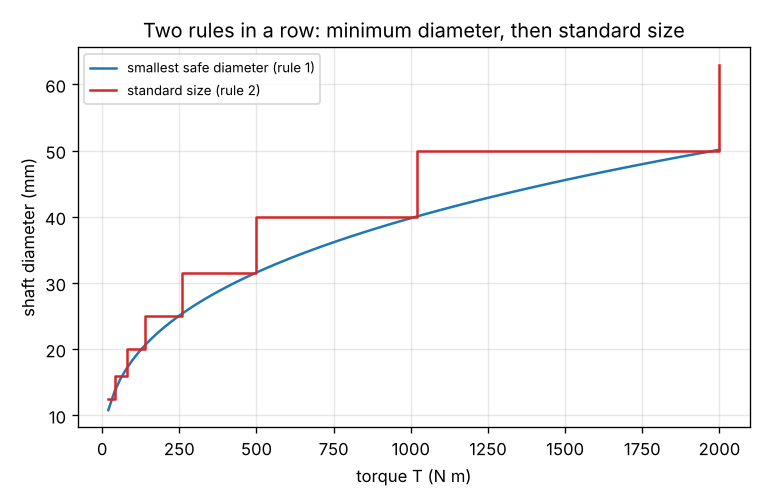
\includegraphics[width=0.78\textwidth]{figures/s01_diameter_vs_torque.png}\caption{Smallest safe diameter (curve) and standard size (steps) against the torque.}\end{figure}

\begin{figure}[h]\centering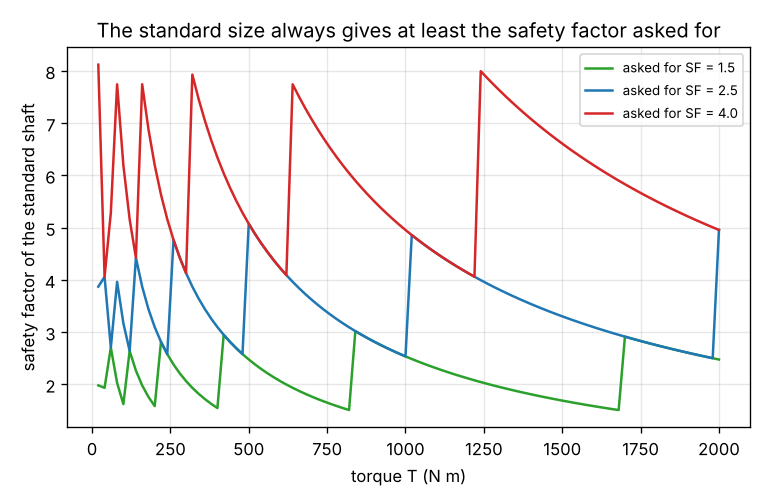
\includegraphics[width=0.78\textwidth]{figures/s01_safety_factor.png}\caption{Safety factor of the standard shaft against the torque, for three requested values.}\end{figure}

\subsection*{E. Worked example}
\textbf{Problem.} A shaft must carry 200 N m. The steel has a tensile yield strength of 350 MPa and the safety factor is 2.5. Find the smallest safe diameter, the standard size, and the stress and safety factor of that shaft.

\begin{enumerate}[nosep]
\item Allowable shear stress: tau\_allow = 0.577 x 350 / 2.5 = 80.8 MPa.
\item Smallest diameter: d\_min = (16 x 200 000 / (pi x 80.8))\textasciicircum{}(1/3) = 23.28 mm.
\item Standard size: the next R10 size not below 23.28 mm is 25 mm (the one below is 20 mm, which is too small).
\item Check: tau = 16 x 200 000 / (pi x 25\textasciicircum{}3) = 65.2 MPa, which is below 80.8 MPa.
\item Safety factor actually obtained: 0.577 x 350 / 65.2 = 3.10, a little above the 2.5 asked for, because we rounded up by 7 percent.
\item Mass per metre of the shaft: 7850 x pi / 4 x 0.025\textasciicircum{}2 = 3.85 kg/m.
\end{enumerate}
\textbf{Answer.} The rules give d\_min = 23.28 mm and a standard shaft of 25 mm, which carries 200 N m with a safety factor of 3.10.

\section{Session 2: When two rules disagree the stricter one wins: strength, stiffness and material}

\subsection*{A. Real-world problem}
A bracket sticks out from a wall and carries a load at its tip. It must not break (strength) and it must not sag more than a given amount (stiffness). Each requirement gives its own minimum thickness, and the plate that is sold comes in fixed thicknesses. Which rule decides, does it change when the bracket gets longer, and is a steel or an aluminium bracket lighter? Take a load of 500 N at 200 mm from the wall, a plate 40 mm wide and at most 1 mm of sag.

\subsection*{B. Concept and theory}
For a plate of width b and thickness t fixed at one end, with a load F at the free end a distance L away, the second moment of area is I = b t\textasciicircum{}3 / 12. The largest bending stress is at the fixing, sigma = M c / I = 6 F L / (b t\textasciicircum{}2), where M = F L and c = t / 2. The strength rule requires sigma not above the allowable stress sigma\_allow = yield / SF, which gives t\_strength = sqrt(6 F L / (b sigma\_allow)). The tip sinks by delta = F L\textasciicircum{}3 / (3 E I) = 4 F L\textasciicircum{}3 / (E b t\textasciicircum{}3), with E the elastic modulus of the material. The stiffness rule requires delta not above delta\_max, which gives t\_stiffness = (4 F L\textasciicircum{}3 / (E b delta\_max))\textasciicircum{}(1/3). The plate must satisfy both, so the required thickness is the larger of the two, and the rule that gives the larger one is the governing rule; then we take the next plate thickness that is sold and check the stress, the sag and the mass b t L rho. Since t\_strength grows with the square root of L and t\_stiffness grows in proportion to L, stiffness governs long brackets and strength short ones; they cross at the critical length. Different materials have different E, yield and density, so the same rules give different plates and masses, and we choose the material with the smallest mass. Aluminium has a third of the elastic modulus of steel but a third of its density, so it needs a thicker plate that can still be lighter. To check the deflection formula independently, we integrate the beam equation E I y'' = M(x) = F (L - x) numerically twice along the plate.

\begin{itemize}[nosep]
\item F: load at the free end (N)
\item L: distance from the wall to the load (mm)
\item b, t: width and thickness of the plate (mm)
\item E: elastic modulus (MPa (N/mm\textasciicircum{}2))
\item sigma\_allow: allowable stress, yield / SF (MPa)
\item delta\_max: largest sag allowed at the tip (mm)
\item rho: density (kg/m\textasciicircum{}3)
\end{itemize}

\[ t_{\text{strength}} = \sqrt{\frac{6\,F\,L}{b\,\sigma_{\text{allow}}}},\qquad t_{\text{stiffness}} = \left(\frac{4\,F\,L^{3}}{E\,b\,\delta_{\max}}\right)^{1/3} \]

\[ t = \max\left(t_{\text{strength}},\,t_{\text{stiffness}}\right),\ \text{then the next plate that is sold} \]

\[ L_c = \left[\left(\frac{6F}{b\,\sigma_{\text{allow}}}\right)^{3/2}\frac{E\,b\,\delta_{\max}}{4F}\right]^{2/3} \]

\subsection*{C. Visual explanation}
The first figure shows the thickness from each rule against the length for the steel bracket. The strength rule (curved) is above the stiffness rule (straight-ish) for short brackets and below it for long ones; the dotted line marks the critical length of about 125 mm. The second figure plots the mass of the standard plate for steel and aluminium against the length: aluminium is lighter at all the lengths shown, and both curves jump when the next plate size is needed.

\begin{figure}[h]\centering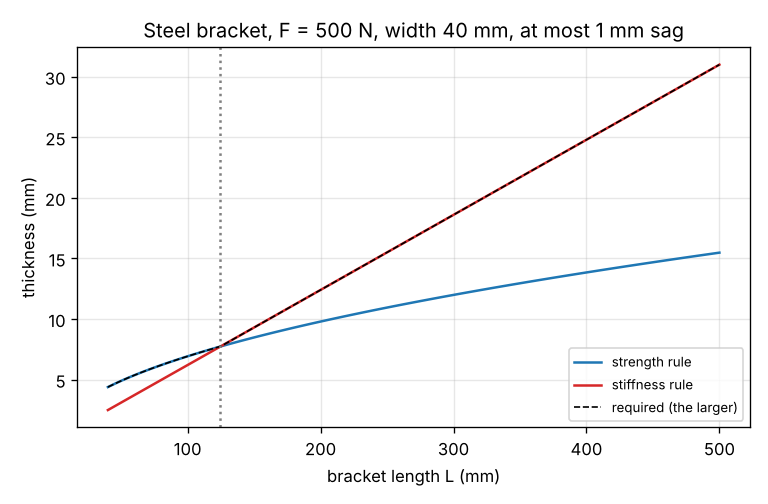
\includegraphics[width=0.78\textwidth]{figures/s02_thickness_vs_length.png}\caption{Thickness from the strength rule and the stiffness rule against the length.}\end{figure}

\begin{figure}[h]\centering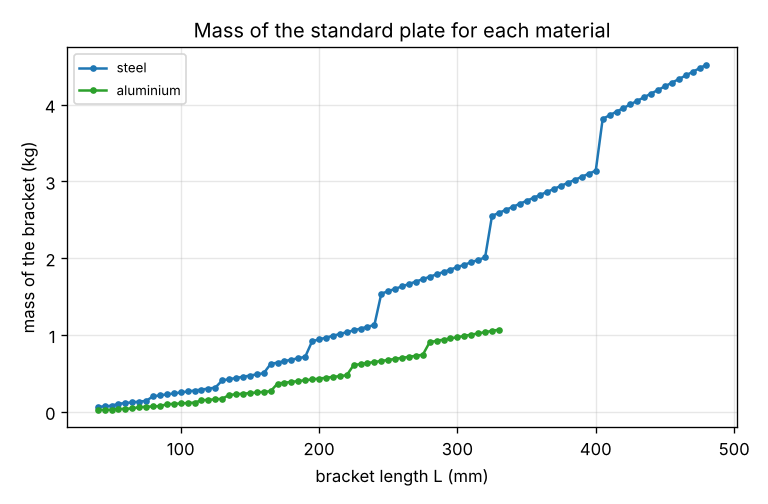
\includegraphics[width=0.78\textwidth]{figures/s02_mass_by_material.png}\caption{Mass of the standard plate against the length, for steel and aluminium.}\end{figure}

\subsection*{E. Worked example}
\textbf{Problem.} A bracket 40 mm wide carries 500 N at 200 mm from the wall and may sag at most 1.0 mm. Take steel with a safety factor of 1.5. Find the thickness from each rule, the plate that is sold, the mass, and the stress and sag of that plate. Then do the same for aluminium.

\begin{enumerate}[nosep]
\item Allowable stress: 235 / 1.5 = 156.7 MPa. Strength: t = sqrt(6 x 500 x 200 / (40 x 156.7)) = 9.78 mm.
\item Stiffness: t = (4 x 500 x 200\textasciicircum{}3 / (210 000 x 40 x 1.0))\textasciicircum{}(1/3) = 12.40 mm. The larger value is 12.40 mm, so stiffness governs.
\item The next plate that is sold is 15 mm. Mass: 40 x 15 x 200 x 7850 x 1e-9 = 0.942 kg.
\item Check the plate: stress 6 x 500 x 200 / (40 x 15\textasciicircum{}2) = 67 MPa (below 157) and sag 4 x 500 x 200\textasciicircum{}3 / (210 000 x 40 x 15\textasciicircum{}3) = 0.56 mm (below 1.0).
\item Aluminium: strength gives 9.68 mm and stiffness gives 17.96 mm (E is only 69 GPa), so the plate is 20 mm, with a mass of 0.432 kg, a sag of 0.72 mm and a stress of 38 MPa.
\item The lightest is aluminium: 0.432 kg against 0.942 kg, even though its plate is thicker.
\end{enumerate}
\textbf{Answer.} Steel needs a 15 mm plate of 0.942 kg (stiffness governs); aluminium needs a 20 mm plate of 0.432 kg, less than half, so the lightest bracket is aluminium.

\section{Session 3: Rules as data: ordering them, catching loops and drawing the part}

\subsection*{A. Real-world problem}
A pipe flange joins two pipes with a ring of bolts. How many bolts it needs depends on the load and the bolt size, the size of the bolt circle depends on the number of bolts and on the pipe, the outside diameter depends on the bolt circle, and so on. A designer keeps all this in a list of rules. If the load doubles, the whole flange should be regenerated. Which rule has to be evaluated first, how do we notice a rule that depends on itself, and how do we know the drawing agrees with the numbers? Take a load of 60 kN, M12 bolts and a pipe of 114.3 mm outside diameter.

\subsection*{B. Concept and theory}
A rule is a name and an equation in text, for example ('n', 'max(4, 2 * ceil(n\_min / 2))'). The names in the equation are its dependencies; each is either an input (load, bolt size, pipe diameter) or another rule. The evaluator accepts only numbers, names, + - * / **, brackets and a short list of functions (sqrt, ceil, max, min and a lookup for the bolt pitch), so a list of rules from a file can never run arbitrary code. The rules may be written in any order, but a rule can be evaluated only after all the rules it depends on. The engine finds an order by a topological sort: repeatedly take the first rule whose dependencies are all available. If rules are left and none can be taken, they depend on each other in a circle and no order exists; the engine must then stop and name the circle (for example a -> b -> c -> a) instead of looping for ever. It must also refuse names that nobody defines, two rules with the same name and rules that overwrite an input. The flange rules are textbook rules of thumb: the hole is 2 mm wider than the bolt; the thread's tensile stress area is pi / 4 (M - 0.9382 pitch)\textasciicircum{}2; a bolt carries area x 320 MPa; the number of bolts is the load divided by that, rounded up to an even number of at least 4; the bolt circle is the larger of pipe + 4 M and the size that keeps the bolts 2.5 M apart; the flange is 3 M wider than the bolt circle; the thickness grows with the bolt size, the pipe and the load; and the mass is the density times the material area times the thickness. Last, the part is drawn as an SVG picture. To check that the drawing and the mass formula describe the same part, we measure the area from the drawing by laying a fine grid over it and counting the grid points inside the ring and outside every hole.

\begin{itemize}[nosep]
\item load: force the flange must carry through its bolts (kN)
\item M: bolt size (nominal diameter) (mm)
\item od: outside diameter of the pipe, which is the bore of the flange (mm)
\item n: number of bolts (even, at least 4) (no unit)
\item pcd: diameter of the bolt circle (mm)
\item fod: outside diameter of the flange, pcd + 3 M (mm)
\item t: thickness of the flange (mm)
\item area\_b: tensile stress area of one bolt (mm\textasciicircum{}2)
\end{itemize}

\[ n = \max\left(4,\ 2\left\lceil \tfrac12 \left\lceil \frac{\mathrm{load}}{A_b\,\sigma_b} \right\rceil \right\rceil\right),\qquad A_b = \frac{\pi}{4}\left(M - 0.9382\,p\right)^{2} \]

\[ p_{cd} = \max\left(\mathrm{od} + 4M,\ \frac{2.5\,M\,n}{\pi}\right),\qquad f_{od} = p_{cd} + 3M \]

\[ m = \rho\,t\left[\frac{\pi}{4}\left(f_{od}^{2} - \mathrm{od}^{2}\right) - n\,\frac{\pi}{4}\,(M+2)^{2}\right] \]

\subsection*{C. Visual explanation}
The first figure shows four flanges produced by the same list of rules for loads of 30, 90, 180 and 300 kN: more bolts as the load grows, and a bolt circle that stays the same because the pipe, not the bolts, sets it. The second figure plots the number of bolts (steps) and the mass (dashed lines) against the load for three bolt sizes: larger bolts need fewer bolts but a thicker, heavier ring.

\begin{figure}[h]\centering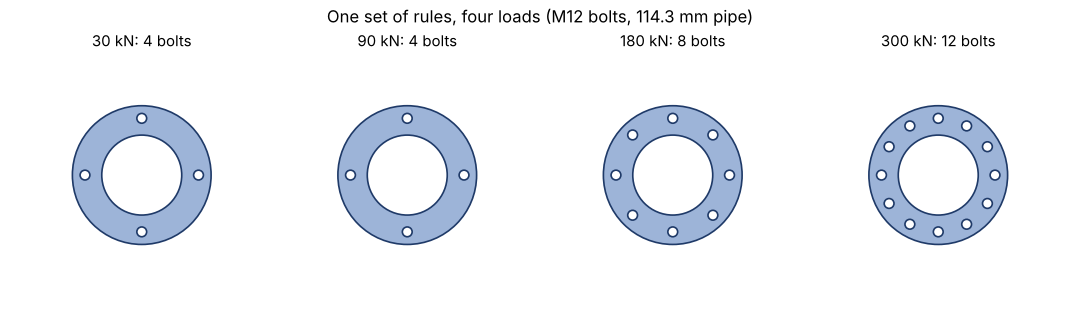
\includegraphics[width=0.78\textwidth]{figures/s03_flange_family.png}\caption{Four flanges generated by the same rules for loads of 30, 90, 180 and 300 kN.}\end{figure}

\begin{figure}[h]\centering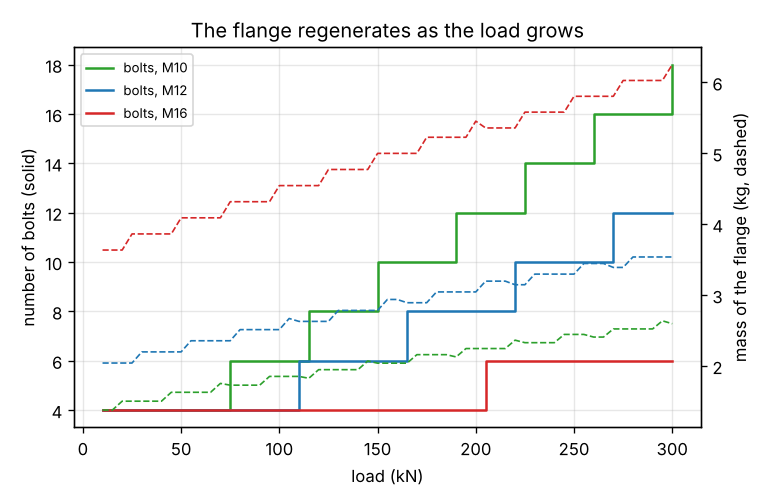
\includegraphics[width=0.78\textwidth]{figures/s03_bolts_vs_load.png}\caption{Number of bolts (steps) and mass (dashed) against the load, for M10, M12 and M16 bolts.}\end{figure}

\subsection*{E. Worked example}
\textbf{Problem.} A flange must carry 60 kN with M12 bolts around a pipe of 114.3 mm outside diameter. Apply the rules in a valid order and find the number of bolts, the bolt circle, the outside diameter, the thickness and the mass.

\begin{enumerate}[nosep]
\item Order found by the engine: t -> area\_b -> f\_bolt -> n\_min -> n -> pcd -> fod -> hole -> mass.
\item Bolt: the stress area is pi / 4 (12 - 0.9382 x 1.75)\textasciicircum{}2 = 84.3 mm2, so one bolt carries 27.0 kN.
\item Number of bolts: 60 / 27.0 = 2.22, rounded up to 3, then to an even number of at least 4: n = 4.
\item Bolt circle: the larger of 114.3 + 4 x 12 = 162.3 mm and 4 x 2.5 x 12 / pi = 38.2 mm, so 162.3 mm. Outside diameter: 162.3 + 36 = 198.3 mm.
\item Thickness: 0.8 x 12 + 0.02 x 114.3 + 0.04 x 60 = 14.3, rounded up to 15 mm. Hole: 14 mm.
\item Mass: area = pi / 4 (198.3\textasciicircum{}2 - 114.3\textasciicircum{}2) - 4 x pi / 4 x 14\textasciicircum{}2 = 20008 mm2, and 7850 x 20008 x 15 x 1e-9 = 2.356 kg.
\item Check: counting grid points in the drawing gives 20005 mm2, within 0.01 percent of the formula.
\end{enumerate}
\textbf{Answer.} The rules give 4 bolts on a 162.3 mm bolt circle, a flange of 198.3 mm outside diameter and 15 mm thickness, and a mass of 2.356 kg.

\section*{Where to go next}
\begin{enumerate}[nosep]
\item \textbf{Units that the rules check.} Give every input and rule a unit (mass, length, force, stress as powers of kg, m and s) and make the engine refuse an equation whose units do not match.
\item \textbf{Tables of standard sizes inside the rules.} Add a lookup function to the engine for tables such as DN to outside diameter, and an interpolation function for a table of stress against temperature.
\item \textbf{Conditional rules and two rings of bolts.} Add a conditional form to the engine and a second ring to the flange when the bolts of one ring would be closer than 2.5 M.
\item \textbf{Explaining a result: why is n = 8?.} Record which values every rule read and print the chain of rules that led to a chosen value, with their equations.
\item \textbf{Searching for the lightest design.} A search over the bolt size and the bracket material that returns the lightest design that passes all checks.
\end{enumerate}

This is a simplified educational model. It is not a validated design tool and must not be used for real structures, electrical installations, vehicles, industrial processes or medical decisions.

\end{document}
